\section{Data, stripping, and simulation}

The data collected by the \lhcb detector used in this thesis totals $3\invfb$; where $1\invfb$ was
collected in the year 2011 with a centre-of-mass energy of $7\tev$, and $2\invfb$ at $8\tev$ was
collected in 2012.
In total, the data collected in 2011 and 2012 is known as Run-1 data.

%\subsection{Stripping}
Even the much reduced \hlttwo output rate of $5\khz$ is a vast amount of data for an
analyst to sift through in a timely manner.
To improve the speed to access data, additional selections are applied to the dataset biannually
which further categorise each event.
This is known as stripping.
Stripped datasets are the only ones accessible to analysts, which makes the process of retrieving
data of interest fast.
Stripping selections in this thesis vary, and will be described when appropriate.


%\section{Simulation}
Reliable analysis of real data would not be possible without selections of simulated events.
%Simulation of events is a vital part of analyses at \lhcb, it allows collaborator's access to pure
These allows collaborator's access to pure samples of specific, requested decays to aid their
research.
This can be for the evaluation of efficiencies, understanding effects in data, or making analysis
decisions without compromising blinded data.
These events are generated in two independent phases: generation and simulation.
Proton-proton collisions are generated using \pythia~\cite{Sjostrand:2006za,*Sjostrand:2007gs}
with a specific \lhcb configuration~\cite{LHCb-PROC-2010-056},
and subsequent hadronic decays are handled by the \evtgen~\cite{Lange:2001uf} package.
The simulation phase is designed to mimic the \lhcb detector's response to particles, this is done
with \geant~\cite{Allison:2006ve,*Agostinelli:2002hh} as described in
Ref.~\cite{LHCb-PROC-2011-006}.
Simulated events after the hadronization stage and before detector modelling are known as
\emph{generator level} simulation.





\begin{figure}
  \begin{center}
    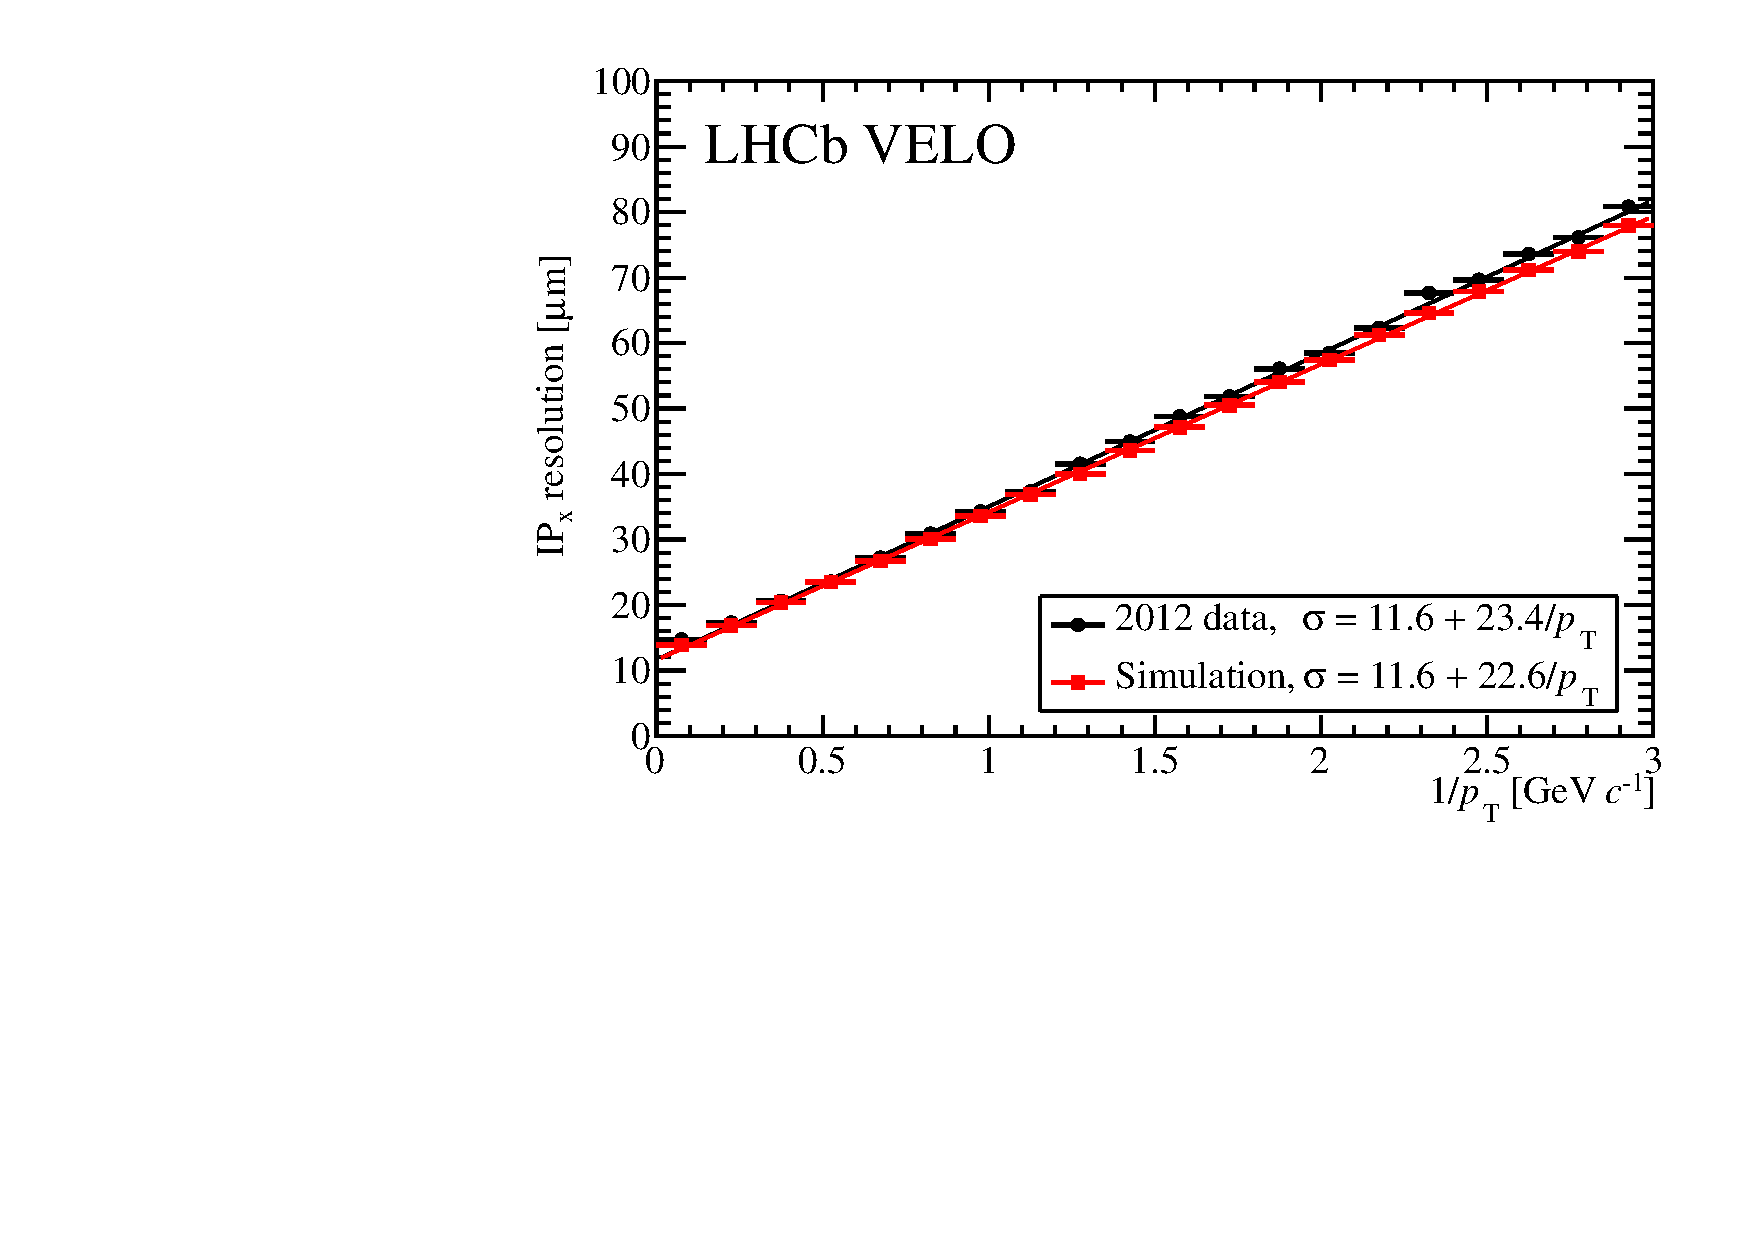
\includegraphics[width=0.48\textwidth]{IPXRes_invp}
    \caption[Impact parameter resolution as a function of inverse momentum comparing data and
    simulation]{
      Impact parameter resolution as a function of a track's inverse momentum comparing (black)
      data taken in 2012 which is also shown in Fig.~\protect\ref{fig:velo:ipres} and (red)
      simulation.  Excellent agreement is seen.
    }
    \label{fig:data:ipres}
  \end{center}
\end{figure}






%%%%%%%%%%%%%%%%%%%%%%%%%%%%%%%%%%%%%%%%%%%%%%%%%%%%%%%%%%%%%%%%%%%%%%%%%%%%%%%%

%The high output rate of the \lhcb trigger means that there is a huge amount of data to be made
%accessible to collaborators, too much to be convenient, in fact.
%Because of \lhcb's wide physics program it is possible to run further collaboration wide selection
%twice a year to reduce the dataset by approximately a factor of ten.
%Within each of these data-subsets further stripping flags are applied which further increase the
%speed which a dataset can be processed.
%The stripping lines used in this thesis are the Dimuon line and the






